\section{Experimenteller Aufbau}

\paragraph{meine Einstellungsparameter:}

\begin{itemize}
    \item Beschleunigungsspannung $U_B$ im Bereich von 12 kV bis 16 kV, zugehöriger Richtungsvektor $\vv{s} = \vektor{1}{0}{0}$
    \item Magnetfeldstärke zweier Ablenkspulen:
    
    \begin{itemize}
        \item $B_1$ im Bereich -5 mT bis 5 mT, zugehöriger Richtungsvektor $\vv{b_1} = \vektor{0}{0}{1}$ % senkrechte Spule
        \item $B_2$ im Bereich -5 mT bis 5 mT, zugehöriger Richtungsvektor $\vv{b_2} = \vektor{0}{1}{0}$ % waagerechte Spule
    \end{itemize}

\end{itemize}

\paragraph{Konstanten:}

\begin{itemize}
    \item Felddurchmesser $d$ = 30 in mm
    \item Masse des Elektrons $m$ =  $9,109 \cdot 10^{-31}$ in kg
    \item Ladung des Elektrons $e$ = $1,602 \cdot 10^{-19}$ in As
    \item Bildschirmabstand $l$ = 500 in mm
\end{itemize}

\paragraph{meine zu berechnenden Parameter:}

\begin{itemize}
    \item Teilchengeschwindigkeit v in $\frac{km}{s}$
    \item Ergebnisvektor $\vv{v}$
    \item Bahnradius r in mm 
    \item alpha $\alpha$
    \item Ablenkungsrichtung $\vv{a}$
\end{itemize}

\section{Berechnung der Elektronenkanone}
Das ist im Strahl und hier wird die Geschwindigkeit berechnet mit welcher dieser aus der Elektronenkanone kommt. 

\subsection{physikalische Erklärung:}

Durch den glühelektrischen Effekt werden Elektronen freigesetzt. Dabei wird ein "Wehnelt-Zylinder" durch eine Heizspannung $U_H$ erhitzt. Die nun freien Elektronen werden durch die Kathode (positiver Pol) gebündelt. Dies geschieht dadurch das in der Mitte der Platte ein kleines Loch vorhanden ist durch welches der Elektronenstrahl nun fließt. Um die Geschwindigkeit zu bestimmen muss der Energieerhaltungssatz betrachtet werden. Dabei wird die kinetische Energie und die elektrische Energie gleichgesetzt. Um die elektrische Energie benutzen zu können, wird das Ende des "Wehnelt-Zylinder" als Anode aufgefasst( negativer Pol) und dadurch entsteht ein elektrisches Feld in welchem auch die elektrische Energie vorhanden ist. 
$$ E_{kin} = E_{el}$$
$$ \frac{1}{2} \cdot m \cdot v^2 = e \cdot U_B$$
Diese Formel wird  nun nach v umgestellt:
\subsection{Die physikalische Formel:} 
$$ v = \sqrt{\frac{2 \cdot e \cdot U_B}{m}}$$

\subsection{Erklärung/Umsetzung der Physik im Code:}

Im Folgenden ist der Code in der Simulation dargestellt. Zu sehen ist, dass die oben genannte Formel benutzt wird und die jeweiligen Attribute aus den zugehörigen Klassen geholt werden. Hier muss sich die Spannung $U_B$ aus der Elektronenkanone (\lstinline$quelle$)  geholt werden. Des Weiteren wird die Spannung mit 1000 multipliziert, da in der Formel mit V gerechnet wird, während die Spannung der Elektronenkanone in kV angegeben ist. Deswegen muss diese noch umgerechnet werden.
\begin{lstlisting}
teilchengeschwindigkeit 
  = Math.sqrt(2 
  * elektronenladung 
  * quelle.spannung 
  * 1000 
  / elektronenmasse);
\end{lstlisting}

\section{Lorentzkraft und Ablenkung}

Das ist im Magneten und hier wird die Ablenkung berechnet.
\begin{figure}
    \centering
    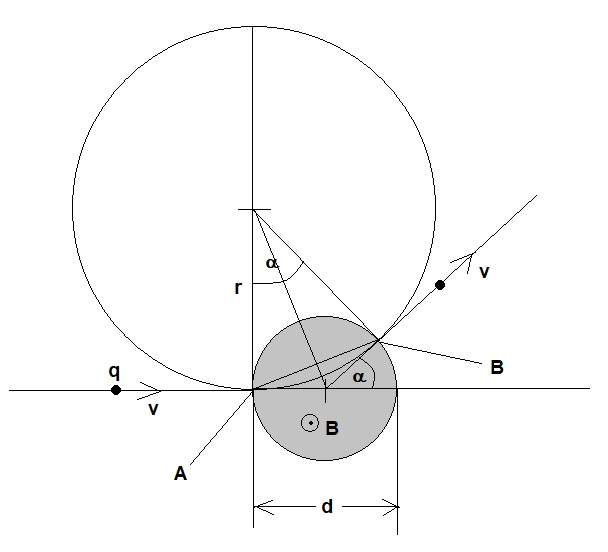
\includegraphics[width=.75\textwidth]{fig/elektronenstrahl-ablenkung_101.jpg}
    \caption{Skizze für Winkelberechnung}
    \label{fig:ausBlock}
\end{figure}

\subsection{physikalische Erklärung:}
Den Radius $r$ wird dadurch berechnet, dass die Lorentzkraft und die Zentripetalkraft gleichgestellt werden. Dies kann so gemacht werden, da die Lorentzkraft die magnetische Kraft darstellt, welche im Magnetfeld vorherrscht. Die Zentripetalkraft hingegen kann benutzt werden, weil die Elektronen im Magnetfeld auf einer Kreisbahn abgelenkt werden, welche durch die Zentripetalkraft dargestellt wird. Dadurch leitet sich ab:
$$ F_m=F_z$$
$$ e \cdot v \cdot B = \frac{m \cdot v^2}{r}$$
Dies lässt sich nun nach $r$ umstellen und man erhält die Formel \ref{eq:r}. Die Formel (2) hingegen lässt sich dadurch herleiten, dass wie in Abbildung \ref{fig:ausBlock} zu sehen ist, durch Trigonometrie der Winkel $\alpha$ herleiten lässt. Durch die Abbildung \ref{fig:ausBlock} wird allerdings nur $\frac{\alpha}{2}$ errechenbar. Durch den Tangens von der Gegenkathete( $ \frac{d}{2}$) und der Ankathete ($ r $) lässt sich $ \frac{\alpha}{2}$ herleiten. Bei Formel (3) wird die Ablenkungsrichtung des Strahls berechnet. Da die linken Hand regel, welche für einen positiven Ladungsträger vorgesehen ist, unserer Ladungsträger(Elektronen) allerdings negativ sind, muss eben jener umgedreht werden und dies wird durch die Multiplikation mit $ -1 $ erreicht. Darauf folgend muss das Kreuzprodukt mit dem Vektor des Magnetfeldes genommen werden.  

\subsection{Die physikalische Formel:}
%\url{https://www.physikerboard.de/ptopic,342494.html#342494}
\begin{equation}
     \label{eq:r}
     r = \frac{m \cdot v}{e \cdot B}
\end{equation}

\begin{equation}
    \label{eq:tan}
    \tan(\frac{\alpha}{2}) = \frac{d}{2 \cdot r}
\end{equation}

\begin{equation}
    \label{eq:a}
    \vv{a} = \vv{s} \cdot (-1) \times \vv{b}
\end{equation}

\subsection{Erklärung/Umsetzung der Physik im Code:}

Im Folgenden ist der Code in der Simulation dargestellt. Hier wird zuerst ebenfalls der \lstinline$Bahnradius$ berechnet, dies geschieht dadurch, dass die Elektronenmasse und die zuvor berechnete Teilchengeschwindigkeit mit aus dem Strahl geholt werden und miteinander multipliziert werden. Des Weiteren wird dieses Ergebnis durch die Elektronenladung und der Magnetfeldstärke mal 1000 dividiert. Die Elektronenladung wird sich ein weiteres mal aus der Klasse Strahl geholt, wo sie gespeichert wurde. Bei der Berechnung des Winkels $\alpha$ wird die oben %Verweis möglich?
bereits genannte Formel mit zwei multipliziert da auf der Ausgabe der tatsächliche Winkel $\alpha$ zu sehen sein soll. Des Winkel $\alpha$ wird im Bogenmaß berechnet. Bei der \lstinline$Ablenkungsrichtung$ wird der Richtungsvektor des Strahl mit $-1$ multipliziert und danach das Kreuzprodukt mit dem Richtungsvektor des Ablenkspulenpaars genommen. Durch den Befehl \lstinline$this.richtungsvektor$ wird auf den Richtungsvektor des jeweiligen Magnetes verwiesen. Des Weiteren ist noch hinzuzufügen, dass die Berechnung jedes Ablenkspulenpaar für sich macht uns daher auch eigene Werte für \lstinline$alpha$, den \lstinline$Bahnradius$ und die \lstinline$Ablenkungsrichtung$ hat.
\begin{lstlisting}
bahnradius
  = strahl.elektronenmasse
    * strahl.teilchengeschwindigkeit
    / (strahl.elektronenladung * magnetfeldstaerke/1000)
    * 1000;
alpha = 2 * Math.atan(felddurchmesser/ (2 *bahnradius ));
ablenkungsrichtung
  = strahl.quelle.richtungsvektor.
    multiplizieren(-1).
    kreuzprodukt(this.richtungsvektor);
\end{lstlisting}

\section{Geometrische Bestimmung des Winkels}

Hier wird der Punkt auf dem Bildschirm berechnet.
\subsection{physikalische Erklärung:}
\subsection{Die physikalische Formel:}
$$ \vv{v} = \vv{v} + \vv{a} \cdot l \cdot \tan(\alpha)$$
\subsection{Erklärung/Umsetzung der Physik im Code:}
\begin{lstlisting}
Vektor ergebnisvektor 
  = new Vektor(bildschirmabstand,0,0);
    for(Magnet m : getWorld().getObjects(Magnet.class) )
        {
            ergebnisvektor 
            = ergebnisvektor.addieren( m.ablenkungsrichtung.
            multiplizieren(bildschirmabstand).
            multiplizieren(Math.tan(m.alpha)));
        }
    return ergebnisvektor;
\end{lstlisting}

\begin{tabular}{c|c|c}
     Formel Buch & Formel Block & Anmerkungen  \\
     \hline
    $\alpha = \frac{d}{r}$ &$\tan(\frac{\alpha}{2}) = \frac{d}{2\cdot r}$& wegen Kleinwinkelnäherung bei dem Buch \\
    \hline
   $r = \frac{m\cdot v}{q\cdot B}$  & $r = \frac{m\cdot v}{q\cdot B}$& alles gleich 
     
\end{tabular}













 
